%&<tex>
\documentclass[notheorems,xcolor=dvipsnames]{beamer}
% \usetheme{metropolis}
\usetheme{Rochester}
%\usefonttheme{serif}

%\usepackage[hmargin=2.5cm, vmargin=2cm]{geometry}
\usepackage{amssymb, mathtools, yhmath, graphicx}
\usepackage{standalone}
\usepackage[most]{tcolorbox}
%\usepackage{fontspec, type1cm, titlesec, titling, fancyhdr, tabularx}
%\usepackage{unicode-math}
\usepackage{float}
\usepackage{transparent}
\usepackage[normalem]{ulem}
\usepackage{bm}
\usepackage{array}
\usepackage{csquotes}
\usetikzlibrary{arrows}
\usepackage{soul}
\usepackage[normalem]{ulem}
\usepackage{tipa}

%\usepackage{eulervm}

\usepackage{xpatch}
\usepackage{relsize}
\usepackage{scalerel}
\usepackage{stackengine}
\usepackage{gauss}
%\usepackage[abbreviations, per-mode=symbol]{siunitx}
\usepackage[CheckSingle, CJKmath]{xeCJK}
\usepackage{fontspec}
\defaultfontfeatures{Mapping=tex-text}
\usefonttheme{professionalfonts}
\usepackage{concmath}
%\usepackage{CJKulem}
%\usepackage{enumitem}
\usepackage{tikz}
\usetikzlibrary{calc, fit, backgrounds}
\usetikzlibrary{tikzmark}
\tikzset {
  overlay node/.style={
    anchor=base, outer sep=0mm, inner sep=0mm,
  }
}
\usepackage{minted}
\usepackage{python}
\usepackage{algorithm2e}
\definecolor{mgray}{rgb}{0.85, 0.85, 0.85}
\colorlet{mgreen}{green!70!black}
\newmintinline{cpp}{bgcolor=mgray}
\def\codesize{\fontsize{9}{12}\selectfont}
\setmonofont[Mapping=]{Source Code Pro}
%\setmonofont[Contextuals={Alternate}]{Fira Code}
\setminted{fontsize=\codesize, linenos, frame=lines, mathescape, autogobble}
%\usemintedstyle{monokai}
%\usepackage{circuitikz}
%\setCJKmainfont[BoldFont=cwTex Q Hei]{cwTex Q Ming}
%\setCJKsansfont[BoldFont=cwTex Q Hei]{cwTex Q Ming}
%\setCJKmonofont[BoldFont=cwTex Q Hei]{cwTex Q Ming}
\setCJKmainfont[AutoFakeSlant,BoldFont=Source Han Sans TW Bold]{Noto Sans CJK TC}
\newfontfamily\SHSTW{Source Han Sans TW}

\def\ofootnotesize{\fontsize{8}{12}}
\def\footnotesize{\fontsize{6}{8}\selectfont}
%\def\normalsize{\fontsize{12}{18}\selectfont}
%\def\large{\fontsize{14}{21}\selectfont}
%\def\Large{\fontsize{16}{24}\selectfont}
%\def\LARGE{\fontsize{18}{27}\selectfont}
%\def\huge{\fontsize{20}{30}\selectfont}

%\titleformat{\section}{\bf\Large}{\arabic{section}}{24pt}{}
%\titleformat{\subsection}{\large}{\arabic{subsection}.}{12pt}{}
%\titlespacing*{\subsection}{0pt}{0pt}{1.5ex}

%\usepackage{parskip}
%\parindent=24pt
%\parskip=1em

\setlength{\parskip}{\baselineskip} 
\usepackage{trimclip}
\DeclareRobustCommand\Longrightarrow{\NewRelbar\joinrel\Rightarrow}
\DeclareRobustCommand\Longleftarrow{\Leftarrow\joinrel\NewRelbar}

\makeatletter
\DeclareRobustCommand\NewRelbar{%
  \mathrel{%
    \mathpalette\@NewRelbar{}%
  }%
}
\newcommand*\@NewRelbar[2]{%
  % #1: math style
  % #2: unused
  \sbox0{$#1=$}%
  \sbox2{$#1\Rightarrow\m@th$}%
  \sbox4{$#1\Leftarrow\m@th$}%
  \clipbox{0pt 0pt \dimexpr(\wd2-.6\wd0) 0pt}{\copy2}%
  \kern-.2\wd0 %
  \clipbox{\dimexpr(\wd4-.6\wd0) 0pt 0pt 0pt}{\copy4}%
}
\makeatother



\newcommand{\img}{\mathsf{i}}
\newcommand{\ex}{\mathsf{e}}
\newcommand{\dD}{\mathrm{d}}
\newcommand{\dI}{\,\mathrm{d}}
\newcommand{\linearprog}[3][maximize]{%
\begin{array}{rl}
  \text{#1} & \kern 1em {#2} \\[8pt]
  \text{subject to} & {\renewcommand\arraystretch{1.1} #3}
\end{array}%
}

\newcommand\abs[1]{\left\lvert #1 \right\rvert}
\newcommand{\ord}{\mathcal{O}}
\newcommand{\fourier}{\mathcal{F}}
\newcommand*{\defeq}{\triangleq}
\renewcommand*{\sharp}{\mathlarger{\#}}
\newcommand*{\bZ}{\mathbb{Z}}
\newcommand*{\bF}{\mathbb{F}}
\newcommand*{\correspond}{\mathrel{\stackon[1.5pt]{=}{\stretchto{%
    \scalerel*[\widthof{=}]{\wedge}{\rule{1ex}{3ex}}}{0.5ex}}}}
\newcommand*{\Expect}{{\rm I\kern-.3em E}}
\newcommand{\btitle}[1]{{\secname} -- #1}
\newcommand{\ctitle}[1]{{\subsecname} -- #1}
\newcommand{\disskip}[1][1]{\vspace*{-#1\parskip}}%
\renewcommand*{\sharp}{\mathlarger{\#}}
\newcommand{\tikzoverlay}[2]{\tikz[baseline, remember picture]{ \node[overlay node] (#1) {#2}}}%

\DeclareMathOperator*{\argmax}{arg\,max}

\theoremstyle{definition}
\newtheorem{theorem}{定理}
\newtheorem{lemma}{引理}
\newtheorem{property}{性質}
\newtheorem{corollary}{推論}
\newtheorem{conjecture}{猜想}
\newtheorem{problem}{題目}

%\colorlet{origintitlefg}{block title.fg}
%\setbeamercolor{origintitle}{use=block,fg=block title.fg,bg=block title.bg}
%\setbeamercolor{originbody}{use=block body,fg=block body.fg,bg=block body.bg}

\newtheorem{definition}{定義}
\BeforeBeginEnvironment{definition}{%
  \setbeamercolor{block title}{fg=white,bg=red!70!black}
  \setbeamercolor{block body}{fg=black, bg=block title.bg!10!bg}
}
\AfterEndEnvironment{definition}{
    \setbeamercolor{block title}{use=structure,fg=white,bg=structure.fg!75!black}
    \setbeamercolor{block body}{parent=normal text,use=block title,bg=block title.bg!10!bg}
}

\newenvironment{missue}{%
\setbeamercolor{block title}{bg=ForestGreen,fg=white}
\setbeamercolor{block body}{bg=blue!20!green!20,fg=black}
\begin{block}{\centering 問題}}{\end{block}}

\newenvironment{exercise}{%
\setbeamercolor{block title}{bg=ForestGreen,fg=white}
\setbeamercolor{block body}{bg=blue!20!green!20,fg=black}
\begin{block}{習題}}{\end{block}}

\renewenvironment{proof}{%
\begin{tcolorbox}[frame empty] {\bf 證明:}\ }{\end{tcolorbox}}

%\setbeamercovered{transparent}
%\usefonttheme[onlymath]{serif}
%\settowidth{\leftmargini}{\usebeamertemplate{itemize item}}

%\makeatletter
%\patchcmd\beamer@@tmpl@frametitle{\insertframetitle}{\insertsection-\insertframetitle}{}{}
%\makeatother

\setbeamertemplate{enumerate item}{%
  \usebeamercolor[bg]{item projected}%
  \raisebox{0.28ex}{\colorbox{bg}{\color{fg}\scriptsize\insertenumlabel}}%
}

\setbeamertemplate{itemize item}{%
  \usebeamercolor[bg]{item projected}%
  \raisebox{0.25ex}{\scriptsize$\blacksquare$}%
}

\AtBeginSection[]{
  \begin{frame}
  \vfill
  \centering
  \begin{beamercolorbox}[sep=6pt,center,shadow=true,rounded=true]{title}
    \usebeamerfont{title}\LARGE\insertsectionhead\par%
  \end{beamercolorbox}
  \vfill
  \end{frame}
  \begin{frame}
    \tableofcontents[currentsection,hideothersubsections]
  \end{frame}
}

\AtBeginSubsection[]{
  \begin{frame}
  \vfill
  \centering
  \begin{beamercolorbox}[sep=6pt,center,shadow=true,rounded=true]{title}
    \usebeamerfont{title}\LARGE\insertsubsectionhead\par%
  \end{beamercolorbox}
  \vfill
  \end{frame}
}

\SetKw{Continue}{continue}
\SetKw{Break}{break}

\makeatletter
\let\save@measuring@true\measuring@true
\def\measuring@true{%
  \save@measuring@true
  \def\beamer@sortzero##1{\beamer@ifnextcharospec{\beamer@sortzeroread{##1}}{}}%
  \def\beamer@sortzeroread##1<##2>{}%
  \def\beamer@finalnospec{}%
}
\makeatother

\title{進階圖論 Advanced Graph Theory}
\author{塗大為}

\renewcommand*{\emph}[1]{{\bfseries #1}}

\begin{document}

\begin{frame}
  \titlepage
\end{frame}

\begin{frame}{講義勘誤}
  \begin{itemize}
    \item Page 218:
      \begin{lemma}
        對於 $T$ 上的兩個節點 $x < y$,任何 $x$ 到 $y$ 的路徑都會包含 $x$ 與 $y$ 在 $T$ 上的一個共同祖先。
      \end{lemma}
    \item Page 250:
      \begin{lemma}[基底的強交換性(Strong Basis Exchange)]
        令 $B_1$ 與 $B_2$ 是 $M$ 中的基底且 $B_1 \neq B_2$,則對於所有 $x \in B_1 \setminus B_2$,存在 $y \in B_2 \setminus B_1$ 使得 $(B_1 \setminus \{x\}) \cup \{y\}$ 與
        $(B_2 \setminus \{y\}) \cup \{x\}$ 都是基底。
    \end{lemma}
  \end{itemize}
\end{frame}

\begin{frame}{講師簡介}
  \begin{itemize}
    \item 塗大為
    \item 臺大資工大四
    \item waynetuinfor/waynetu
    \item ICPC: waynedisonitau123
      \begin{itemize}
        \item 臺大 2020, 2021 World Finals 代表隊
        \item 半退休狀態
      \end{itemize}
    \item 因為想要學習圖論所以當圖論講師
  \end{itemize}
\end{frame}

\begin{frame}{大綱}
  \tableofcontents[hideallsubsections]
\end{frame}

\documentclass[standalone]{beamer}

\begin{document}

\section{進階經典算法}

\subsection{支配樹}

\newcommand{\idom}{\operatorname{idom}}
\newcommand{\sdom}{\operatorname{sdom}}
\newcommand{\dom}{\operatorname{dom}}

\begin{frame}{\ctitle{Motivation}}
  \onslide<1-> {
    \begin{problem}[Useful Roads]
      給一個 $n$ 點 $m$ 邊的有向圖,求出所有有用的邊。一個邊 $e$ 是有用的若存在一個點 $x$ 使得有
      一條從 $1$ 到 $x$ 的簡單路徑通過 $e$。

      \begin{itemize}
        \item $2 \leq n, m \leq 2 \times 10^5$
      \end{itemize}
    \end{problem}
  }
  \onslide<2-> {
    \begin{figure}[H]
      \centering
      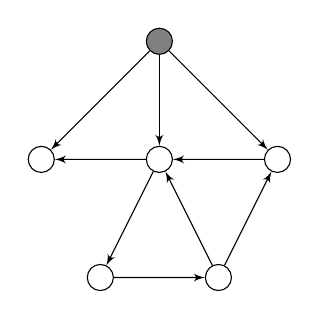
\begin{tikzpicture}[scale=1.5]
        \tikzset{vertex/.style = {shape=circle,draw,minimum size=0.5em}}
        \tikzset{edge/.style = {-,> = latex'}}
        \node[vertex, fill=gray] (1) at (0, 0) {};
        \node[vertex] (2) at (-1, -1) {};
        \node[vertex] (3) at (0, -1) {};
        \node[vertex] (4) at (1, -1) {};
        \node[vertex] (5) at (-0.5, -2) {};
        \node[vertex] (6) at (0.5, -2) {};

        \draw[edge,->] (1) to (2);
        \draw[edge,->] (1) to (3);
        \draw[edge,->] (1) to (4);
        \draw[edge,->] (4) to (3);
        \draw[edge,->] (3) to (2);
        \draw[edge,->] (3) to (5);
        \draw[edge,->] (5) to (6);
        \draw[edge,->] (6) to (3);
        \draw[edge,->] (6) to (4);
      \end{tikzpicture}
    \end{figure}
  }
\end{frame}

\begin{frame}{\ctitle{Definition}}
  \onslide<1-> {
    \begin{definition}
      給定一個有向圖 $G$ 以及源點 $r$,定義節點 $d$ \textbf{支配(dominate)}節點 $x$ 若所有
      $r$ 到 $x$ 的路徑都必須經過 $d$。若 $d \neq x$,則稱 $d$ 嚴格支配 $x$。
    \end{definition}
  }
  \onslide<2-> {
    \begin{definition}
      對於節點 $x \neq r$,$x$ 的\textbf{直接支配者(Immediate Dominator)} $\idom(x)$ 滿
      足

      \begin{itemize}
        \item $\idom(x)$ 支配 $x$ 且 $\idom(x) \neq x$,且
        \item 對於所有支配 $x$ 的 $y \neq x$,$y$ 也支配 $\idom(x)$。
      \end{itemize}
    \end{definition}
  }
\end{frame}

\begin{frame}{\ctitle{Example}}
  \begin{figure}[H]
    \centering
    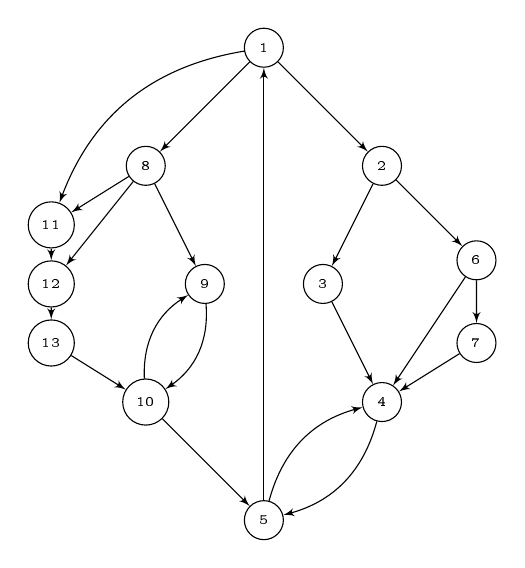
\begin{tikzpicture}[scale=1.5]
      \tikzset{vertex/.style = {shape=circle,draw,minimum size=0.5em}}
      \tikzset{edge/.style = {-,> = latex'}}
      \node[vertex] (r) at (0, 0) {\tiny 1};
      \node[vertex] (b) at (-1, -1) {\tiny 8};

      \node[vertex] (a) at (-1.8, -1.5) {\tiny{11}};
      \node[vertex] (d) at (-1.8, -2) {\tiny{12}};
      \node[vertex] (l) at (-1.8, -2.5) {\tiny{13}};
      \node[vertex] (h) at (-1, -3) {\tiny{10}};
      \node[vertex] (e) at (-0.5, -2) {\tiny 9};

      \node[vertex] (c) at (1, -1) {\tiny 2};
      \node[vertex] (f) at (0.5, -2) {\tiny 3};
      \node[vertex] (i) at (1, -3) {\tiny 4};
      \node[vertex] (g) at (1.8, -1.8) {\tiny 6};
      \node[vertex] (j) at (1.8, -2.5) {\tiny 7};

      \node[vertex] (k) at (0, -4) {\tiny 5};

      \draw[edge,->] (r) to (b);
      \draw[edge,->] (r) to (c);
      \draw[edge,->,bend right=30] (r) to (a);
      \draw[edge,->] (b) to (a);
      \draw[edge,->] (b) to (e);
      \draw[edge,->] (b) to (d);
      \draw[edge,->,bend left=30] (e) to (h);
      \draw[edge,->,bend left=30] (h) to (e);
      \draw[edge,->] (a) to (d);
      \draw[edge,->] (d) to (l);
      \draw[edge,->] (l) to (h);
      \draw[edge,->] (h) to (k);

      \draw[edge,->] (c) to (f);
      \draw[edge,->] (c) to (g);
      \draw[edge,->] (f) to (i);
      \draw[edge,->] (g) to (j);
      \draw[edge,->] (g) to (i);
      \draw[edge,->] (j) to (i);

      \draw[edge,->] (k) to (r);
      \draw[edge,->,bend left=30] (k) to (i);
      \draw[edge,->,bend left=30] (i) to (k);
    \end{tikzpicture}
  \end{figure}
\end{frame}

\begin{frame}{\ctitle{Semi-Dominator}}
  \begin{columns}
    \begin{column}{0.45\textwidth}
      \onslide<1-> {
        \begin{definition}
          對於 $x \neq r$,$x$ 的半支配者 $\sdom(x)$ 為所有 $y$ 使得存在一條
          $y, v_1, v_2, \ldots, v_k, x$ 且所有 $v_i$ 都大於 $x$ 的路徑中,最小的 $y$。
        \end{definition}
      }
    \end{column}
    \begin{column}{0.55\textwidth}
      \onslide<2-> {
        \begin{figure}[H]
          \centering
          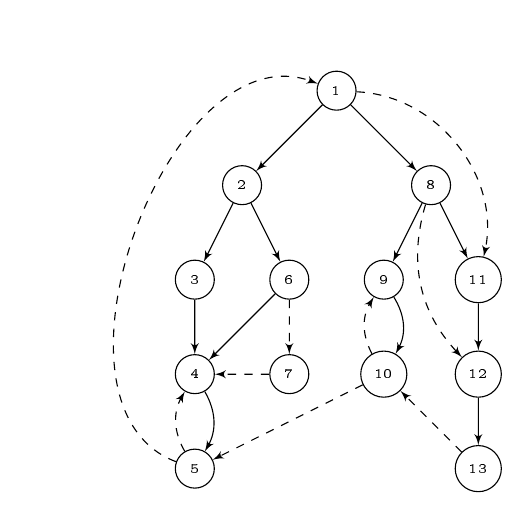
\begin{tikzpicture}[scale=1.2]
            \tikzset{vertex/.style = {shape=circle,draw,minimum size=1em}}
            \tikzset{edge/.style = {-,> = latex'}}

            \node[vertex] (r) at (0, -1) {\tiny 1};

            \node[vertex] (c) at (-1, -2) {\tiny 2};
            \node[vertex] (f) at (-1.5, -3) {\tiny 3};
            \node[vertex] (i) at (-1.5, -4) {\tiny 4};
            \node[vertex] (k) at (-1.5, -5) {\tiny 5};
            \node[vertex] (g) at (-0.5, -3) {\tiny 6};
            \node[vertex] (j) at (-0.5, -4) {\tiny 7};

            \node[vertex] (b) at (1, -2) {\tiny 8};
            \node[vertex] (e) at (0.5, -3) {\tiny 9};
            \node[vertex] (h) at (0.5, -4) {\tiny{10}};
            \node[vertex] (a) at (1.5, -3) {\tiny{11}};
            \node[vertex] (d) at (1.5, -4) {\tiny{12}};
            \node[vertex] (l) at (1.5, -5) {\tiny{13}};

            \draw[edge,->] (r) to (b);
            \draw[edge,->] (r) to (c);
            \draw[edge,->,bend left=50,dashed] (r) to (a);
            \draw[edge,->] (b) to (a);
            \draw[edge,->] (b) to (e);
            \draw[edge,->,dashed,bend right] (b) to (d);
            \draw[edge,->,bend left=30] (e) to (h);
            \draw[edge,->,bend left=30,dashed] (h) to (e);
            \draw[edge,->] (a) to (d);
            \draw[edge,->] (d) to (l);
            \draw[edge,->,dashed] (l) to (h);
            \draw[edge,->,dashed] (h) to (k);

            \draw[edge,->] (c) to (f);
            \draw[edge,->] (c) to (g);
            \draw[edge,->] (f) to (i);
            \draw[edge,->,dashed] (g) to (j);
            \draw[edge,->] (g) to (i);
            \draw[edge,->,dashed] (j) to (i);

            \draw[edge,->,bend left=90,dashed] (k) to (r);
            \draw[edge,->,bend left=30,dashed] (k) to (i);
            \draw[edge,->,bend left=30] (i) to (k);
          \end{tikzpicture}
        \end{figure}
      }
    \end{column}
  \end{columns}
\end{frame}

\begin{frame}{\ctitle{Lemmas}}
  \onslide<1-> {
    \begin{lemma}
      對於 $T$ 上的兩個節點 $x < y$,任何 $x$ 到 $y$ 的路徑都會包含 $x$ 與 $y$ 在 $T$ 上的一個共同祖先。
    \end{lemma}
  }
  \onslide<2-> {
    \begin{lemma}
      對於 $x \neq r$,$\sdom(x)$ 是 $x$ 在 $T$ 上的祖先且 $\sdom(x) \neq x$。
    \end{lemma}
  }
  \onslide<3-> {
    \begin{lemma}
      對於 $x \neq r$,$\idom(x)$ 是 $\sdom(x)$ 在 $T$ 上的祖先。
    \end{lemma}
  }
\end{frame}

\begin{frame}{\ctitle{Lemmas}}
  \onslide<1-> {
    \begin{lemma}
      對於 $x \neq r$ 以及 $y \neq r$,若 $x$ 是 $y$ 在 $T$ 上的祖先,則 (1) $x$ 是 $\idom(y)$ 的祖先或 (2) $\idom(y)$ 是 $\idom(x)$ 的祖先。
    \end{lemma}
  }
  \onslide<2-> {
    \begin{lemma}
      對於 $x \neq r$,如果對於所有在 $\sdom(x)$ 與 $x$ 於 $T$ 上的路徑中的節點
      $y \neq \sdom(x)$,都有 $\sdom(y) \geq \sdom(x)$ 的話,則 $\idom(x) = \sdom(x)$。
    \end{lemma}
  }
  \onslide<3-> {
    \begin{lemma}
      對於 $x \neq r$,令 $y$ 為 $\sdom(x)$ 與 $x$ 於 $T$ 上路徑中,有最小 $\sdom(y)$ 的節
      點。則 $\sdom(y) \leq \sdom(x)$ 且 $\idom(x) = \idom(y)$。
    \end{lemma}
  }
\end{frame}

\begin{frame}{\ctitle{Algorithm}}
  \begin{itemize}
    \item 支配者:
      \onslide<2-> {
        \[
          \idom(x) =
            \begin{cases}
              \sdom(x), & \sdom(x) = \sdom(y) \\
              \idom(y), & \sdom(x) \neq \sdom(y) \\
            \end{cases}
        \]
      }
    \item 半支配者:
      \onslide<3-> {
        \[
          \sdom(x) = \min
            \begin{cases}
              y, & (y, x) \in E(G), y < x \\
              \sdom(z), & (y, x) \in E(G), z > x \text{ 是 $y$ 的祖先} \\
            \end{cases}
        \]
      }
  \end{itemize}
\end{frame}

\begin{frame}{\ctitle{Algorithm}}
  \begin{algorithm}[H]
    \KwData{有向圖 $G = (V, E)$、根 $r \in V$}

    從 $r$ 跑一次 DFS 得到 DFS 序列 $v_1, v_2, \ldots, v_n$ \\

    \onslide<2-> {
      \For{$i = n$ \KwTo $1$} {
        $\sdom(v_i) \gets \min\{\sdom(\operatorname{Eval}(u)) \mid (u, v_i) \in E\}$ \\

        \onslide<3-> {
          \For{$u \in \sdom^{-1}(v_i)$} {
            $p \gets \operatorname{Eval}(u)$ \\
            $\dom(u) =
              \begin{cases}
                v_i, & \sdom(p) = x \\
                p, & \sdom(p) \neq x \\
              \end{cases}$ \\
          }
        }

        \onslide<4-> {
          $\operatorname{Link}(v_i, \operatorname{par}(v_i))$
        }
      }
    }

    \onslide<5-> {
      \For{$i = 1$ \KwTo $n$} {
        $\idom(v_i) =
          \begin{cases}
            \dom(v_i), & \sdom(v_i) = \dom(v_i) \\
            \dom(\dom(v_i)), & \sdom(v_i) \neq \dom(v_i) \\
          \end{cases}$
      }
    }
  \end{algorithm}
\end{frame}

\subsection{有向最小生成樹}

\begin{frame}{\ctitle{Motivation}}
  \begin{problem}[GGS-DDU]
    有 $n$ 道關卡,第 $i$ 道有 $0, 1, \ldots, A_i$、共 $A_i + 1$ 個等級。一開始你在每個關
    卡都是 $0$ 等。有 $m$ 個道具,對於第 $i$ 個道具,假如你在第 $c_i$ 關達到至少 $L_{1,i}$
    等的話,那你可以花 $p_i$ 元在第 $d_i$ 關晉升到 $L_{2,i}$ 等。請問要在每一關都達到滿等最少
    需要花多少錢?

    \begin{itemize}
      \item $1 \leq n \leq 50$
      \item $0 \leq m \leq 2000$
      \item $A_i$ 總和不超過 $500$
    \end{itemize}
  \end{problem}
\end{frame}

\begin{frame}{\ctitle{Idea}}
  \begin{figure}[H]
    \centering
    \begin{tikzpicture}[scale=1.5]
      \tikzset{vertex/.style = {shape=circle,draw,minimum size=1em}}
      \tikzset{edge/.style = {-,> = latex'}}
      \node[vertex, fill=gray] (r) at (0, 0) {};
      \node[vertex] (v1) at (1, -1) {};
      \node[vertex] (v2) at (1, -2) {};
      \node[vertex] (v3) at (0, -2) {};
      \node[vertex] (x) at (-1, -1) {};
      \node[vertex] (v4) at (-1, -2) {};
      \node[vertex] (v5) at (-1, -3) {};
      \node[vertex] (v6) at (1, -3) {};

      \only<1> {
        \draw[edge,->] (r) -- (v1) node [midway,right] {$1$};
        \draw[edge,->] (v1) -- (v2) node [midway,left] {$1$};
        \draw[edge,->] (v2) -- (v3) node [midway,below] {$1$};
        \draw[edge,->] (r) -- (x) node [midway,left] {$1$};
        \draw[edge,->] (x) -- (v4) node [midway,left] {$1$};
        \draw[edge,->] (v4) -- (v5) node [midway,left] {$1$};
        \draw[edge,->] (v5) -- (v6) node [midway,above] {$2$};
        \draw[edge,->] (v2) to node [midway,left] {$1$} (v6) ;
        \draw[edge,->] (v3) -- (v4) node [midway,below] {$2$};
        \draw[edge,->,bend right] (v6) to node [midway,right] {$2$} (v1);
      }
      \only<2> {
        \draw[edge,->] (r) -- (v1) node [midway,right] {$2$};
        \draw[edge,->] (v1) -- (v2) node [midway,left] {$1$};
        \draw[edge,->] (v2) -- (v3) node [midway,below] {$1$};
        \draw[edge,->] (r) -- (x) node [midway,left] {$1$};
        \draw[edge,->] (x) -- (v4) node [midway,left] {$2$};
        \draw[edge,->] (v4) -- (v5) node [midway,left] {$1$};
        \draw[edge,->] (v5) -- (v6) node [midway,above] {$1$};
        \draw[edge,->] (v2) -- (v6) node [midway,left] {$2$};
        \draw[edge,->] (v3) -- (v4) node [midway,below] {$1$};
        \draw[edge,->,bend right] (v6) to node [midway,right] {$1$} (v1);
      }
    \end{tikzpicture}
  \end{figure}
\end{frame}

\begin{frame}{\ctitle{Key Lemma}}
  \begin{columns}
    \begin{column}{0.5\textwidth}
      \onslide<1-> {
        \begin{lemma}
          若對於除了 $r$ 以外的點都蒐集它們最小的入邊,而這 $n - 1$ 條邊形成一個環 $C$
          的話,那存在一個最小有向生成樹包含 $C$ 中的 $|C| - 1$ 條邊。
        \end{lemma}
      }
    \end{column}
    \begin{column}{0.5\textwidth}
      \onslide<2-> {
        \begin{figure}[H]
          \centering
          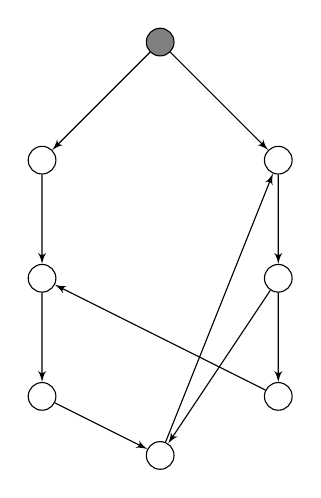
\begin{tikzpicture}[scale=1.5]
            \tikzset{vertex/.style = {shape=circle,draw,minimum size=1em}}
            \tikzset{edge/.style = {-,> = latex'}}
            \node[vertex, fill=gray] (r) at (0, 0) {};
            \node[vertex] (v1) at (1, -1) {};
            \node[vertex] (v2) at (1, -2) {};
            \node[vertex] (v3) at (1, -3) {};
            \node[vertex] (x) at (-1, -1) {};
            \node[vertex] (v4) at (-1, -2) {};
            \node[vertex] (v5) at (-1, -3) {};
            \node[vertex] (v6) at (0, -3.5) {};
            \draw[edge,->] (r) -- (v1);
            \draw[edge,->] (v1) -- (v2);
            \draw[edge,->] (v2) -- (v3);
            \draw[edge,->] (r) -- (x);
            \draw[edge,->] (x) -- (v4);
            \draw[edge,->] (v4) -- (v5);
            \draw[edge,->] (v5) -- (v6);
            \draw[edge,->] (v2) -- (v6);
            \draw[edge,->] (v3) -- (v4);
            \draw[edge,->] (v6) -- (v1);
          \end{tikzpicture}
        \end{figure}
      }
    \end{column}
  \end{columns}
\end{frame}

\begin{frame}{\ctitle{Algorithm}}
  \begin{algorithm}[H]
    \KwData{帶權有向圖 $G = (V, E, w)$、根 $r \in V$}
    \KwResult{$G$ 的有向最小生成樹的權值}

    \onslide<2-> {
      $in(v) \gets$ $v$ 的最小權入邊($v \neq r$) \\
      $G_{in} \gets$ $in(v)$ 所構成的子圖 \\
    }
    \onslide<3-> {
      \If{$G_{in}$ 沒有有向環} {
        \Return $\sum_{v \neq r}w(in(v))$
      }
    }
    \onslide<4-> {
      $C \gets$ $G_{in}$ 中的一個有向環 \\
      $V^\prime \gets (V \setminus V(C)) \cup \{c\}$ \\
      $E^\prime \gets \{(f(u), f(v)) \mid (u, v) \in E\}$ \\
    }
    \onslide<5-> {
      $w^\prime((f(u), f(v))) \gets
        \begin{cases}
          w((u, v)), & v \not\in V(C) \\
          w((u, v)) - w(in(v)) & v \in V(C) \\
        \end{cases}$ \\
    }
    \onslide<6-> {
      \Return $\operatorname{DMST}(G^\prime = (V^\prime, E^\prime, w^\prime), r) + \sum_{v \neq r}w(in(v))$
    }
  \end{algorithm}
\end{frame}

\begin{frame}{\ctitle{Subquadratic Implementation}}
  \begin{tabular}{| c | c | c | c | c |}
    \hline
    & \texttt{top()} & \texttt{pop()} & \texttt{push()} & \texttt{merge()} \\\hline
    Leftist Tree & $O(1)$ & $O(\log{n})$ & $O(\log{n})$ & $O(\log{n})$ \\\hline
    Fibonacci Heap & $O(1)$ & $O(\log{n})$ & $O(1)$ & $O(1)$ \\\hline
    Pairing Heap & $O(1)$ & $O(\log{n})$ & $O(1)$ & $O(1)$ \\\hline
  \end{tabular}

  \begin{itemize}
    \item Library Checker: \url{https://judge.yosupo.jp/problem/directedmst}
  \end{itemize}
\end{frame}

\end{document}

\documentclass[standalone]{beamer}

\begin{document}

\section{匹配}

\subsection{二分圖匹配}

\begin{frame}{\ctitle{Augmenting Path}}
  \onslide<1-> {
    \begin{definition}
      對於一組匹配 $M$,路徑 $P = (x_1, y_1, x_2, y_2, \ldots, x_n, y_n, x_{n + 1})$
      被稱作\textbf{交錯路徑(alternating path)}若以下條件滿足:
      \begin{itemize}
        \item $x_1 \not\in M$
        \item $(y_i, x_{i + 1}) \in M$, $(x_i, y_i) \not\in M$
      \end{itemize}
    \end{definition}
  }
  \onslide<2-> {
    \begin{definition}
      對於一組匹配 $M$,路徑 $P = (x_1, y_1, x_2, y_2, \ldots, x_n, y_n)$
      被稱作\textbf{增廣路徑(augmenting path)}若以下條件滿足:
      \begin{itemize}
        \item $x_1 \not\in M$, $y_n \not\in M$
        \item $(y_i, x_{i + 1}) \in M$, $(x_i, y_i) \not\in M$
      \end{itemize}
    \end{definition}
  }
\end{frame}

\begin{frame}{\ctitle{Key Lemma}}
  \onslide<1-> {
    \begin{theorem}[Berge's Lemma]
      一組匹配 $M$ 為圖 $G$ 中最大匹配若且唯若圖上不存在對於 $M$ 來說的增廣路徑。
    \end{theorem}
  }
  \onslide<2-> {
    \begin{figure}[H]
      \centering
      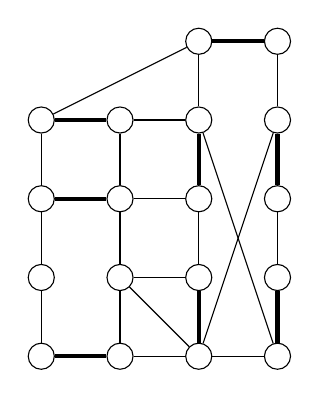
\begin{tikzpicture}[scale=1]
        \tikzset{vertex/.style = {shape=circle,draw,minimum size=0.5em}}
        \tikzset{edge/.style = {-,> = latex'}}
        \node[vertex] (1) at (0, 0) {};
        \node[vertex] (2) at (1, 0) {};
        \node[vertex] (3) at (1, -1) {};
        \node[vertex] (4) at (0, -1) {};
        \node[vertex] (5) at (0, -2) {};
        \node[vertex] (6) at (1, -2) {};
        \node[vertex] (7) at (0, -3) {};
        \node[vertex] (8) at (1, -3) {};
        \node[vertex] (9) at (2, 1) {};
        \node[vertex] (10) at (2, 0) {};
        \node[vertex] (11) at (2, -1) {};
        \node[vertex] (12) at (2, -2) {};
        \node[vertex] (13) at (2, -3) {};
        \node[vertex] (14) at (3, 1) {};
        \node[vertex] (15) at (3, 0) {};
        \node[vertex] (16) at (3, -1) {};
        \node[vertex] (17) at (3, -2) {};
        \node[vertex] (18) at (3, -3) {};

        \draw[edge,ultra thick] (1) to (2);
        \draw[edge] (2) to (3);
        \draw[edge,ultra thick] (3) to (4);
        \draw[edge] (1) to (4);
        \draw[edge] (4) to (5);
        \draw[edge] (3) to (6);
        \draw[edge] (5) to (7);
        \draw[edge] (6) to (8);
        \draw[edge,ultra thick] (7) to (8);

        \draw[edge] (9) to (10);
        \draw[edge,ultra thick] (10) to (11);
        \draw[edge] (11) to (12);
        \draw[edge,ultra thick] (12) to (13);
        \draw[edge] (14) to (15);
        \draw[edge,ultra thick] (15) to (16);
        \draw[edge] (16) to (17);
        \draw[edge,ultra thick] (17) to (18);
        \draw[edge,ultra thick] (9) to (14);
        \draw[edge] (13) to (18);

        \draw[edge] (2) to (10);
        \draw[edge] (3) to (11);
        \draw[edge] (6) to (12);
        \draw[edge] (8) to (13);
        \draw[edge] (1) to (9);
        \draw[edge] (10) to (18);
        \draw[edge] (13) to (15);

        \draw[edge] (6) to (13);
      \end{tikzpicture}
      \hspace{3em}
      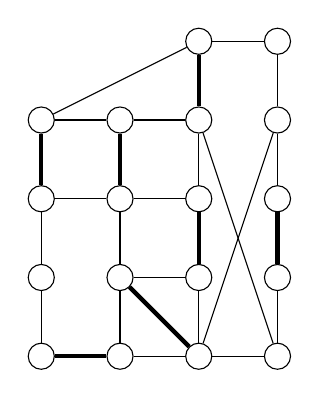
\begin{tikzpicture}[scale=1]
        \tikzset{vertex/.style = {shape=circle,draw,minimum size=0.5em}}
        \tikzset{edge/.style = {-,> = latex'}}
        \node[vertex] (1) at (0, 0) {};
        \node[vertex] (2) at (1, 0) {};
        \node[vertex] (3) at (1, -1) {};
        \node[vertex] (4) at (0, -1) {};
        \node[vertex] (5) at (0, -2) {};
        \node[vertex] (6) at (1, -2) {};
        \node[vertex] (7) at (0, -3) {};
        \node[vertex] (8) at (1, -3) {};
        \node[vertex] (9) at (2, 1) {};
        \node[vertex] (10) at (2, 0) {};
        \node[vertex] (11) at (2, -1) {};
        \node[vertex] (12) at (2, -2) {};
        \node[vertex] (13) at (2, -3) {};
        \node[vertex] (14) at (3, 1) {};
        \node[vertex] (15) at (3, 0) {};
        \node[vertex] (16) at (3, -1) {};
        \node[vertex] (17) at (3, -2) {};
        \node[vertex] (18) at (3, -3) {};

        \draw[edge] (1) to (2);
        \draw[edge,ultra thick] (2) to (3);
        \draw[edge] (3) to (4);
        \draw[edge,ultra thick] (1) to (4);
        \draw[edge] (4) to (5);
        \draw[edge] (3) to (6);
        \draw[edge] (5) to (7);
        \draw[edge] (6) to (8);
        \draw[edge,ultra thick] (7) to (8);

        \draw[edge,ultra thick] (9) to (10);
        \draw[edge] (10) to (11);
        \draw[edge,ultra thick] (11) to (12);
        \draw[edge] (12) to (13);
        \draw[edge] (14) to (15);
        \draw[edge] (15) to (16);
        \draw[edge,ultra thick] (16) to (17);
        \draw[edge] (17) to (18);
        \draw[edge] (9) to (14);
        \draw[edge] (13) to (18);

        \draw[edge] (2) to (10);
        \draw[edge] (3) to (11);
        \draw[edge] (6) to (12);
        \draw[edge] (8) to (13);
        \draw[edge] (1) to (9);
        \draw[edge] (10) to (18);
        \draw[edge] (13) to (15);

        \draw[edge,ultra thick] (6) to (13);
      \end{tikzpicture}
    \end{figure}
  }
\end{frame}

\begin{frame}[fragile]{\ctitle{Algorithm}}
  \begin{minted}[linenos=false]{cpp}
    bool Dfs(int x) {
      for (int y : g[x]) {
        if (visited[y]) continue;
        visited[y] = true;
        if (match[y] == -1 || Dfs(match[y])) {
          // augmenting path found
          match[y] = x;
          return true;
        }
      }
      return false;
    }

    for (int x = 0; x < N; ++x) {
      std::fill(visited.begin(), visited.end(), false);
      Dfs(x);
    }
  \end{minted}
\end{frame}

\begin{frame}{\ctitle{Hopcroft-Karp Algorithm}}
  \begin{corollary}
    對一組匹配 $M$,若最短增廣路徑長度為 $k$,則
    \[ |M^{*}| - |M| \leq O(\frac{1}{k}) \cdot |M^{*}| \]
  \end{corollary}

  \onslide<2-> {
    \begin{algorithm}[H]
      $M \gets \emptyset$ \\
      \While{還有增廣路徑} {
        \onslide<3-> {
          用 BFS 找出最短增廣路距離 $d$ \\
          用 DFS 找出極大的最短增廣路集合 $\mathcal{P}$ \\
          $M \gets M \triangle \mathcal{P}$
        }
      }
    \end{algorithm}
  }
\end{frame}

\subsection{一般圖匹配}

\begin{frame}{\ctitle{Blossom}}
  \onslide<1-> {
    \begin{figure}[H]
      \centering
      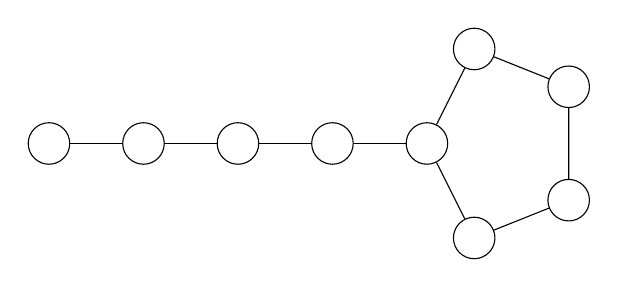
\begin{tikzpicture}[scale=1.2]
        \tikzset{vertex/.style = {shape=circle,draw,minimum size=1.5em}}
        \tikzset{edge/.style = {-,> = latex'}}
        \node[vertex] (a) at (0, 0) {};
        \node[vertex] (b) at (1, 0) {};
        \node[vertex] (c) at (2, 0) {};
        \node[vertex] (d) at (3, 0) {};
        \node[vertex] (e) at (4, 0) {};
        \node[vertex] (f) at (4.5, 1) {};
        \node[vertex] (g) at (5.5, 0.6) {};
        \node[vertex] (h) at (5.5, -0.6) {};
        \node[vertex] (i) at (4.5, -1) {};
        \draw[edge] (a) to (b);
        \draw[edge] (b) to (c);
        \draw[edge] (c) to (d);
        \draw[edge] (d) to (e);
        \draw[edge] (e) to (f);
        \draw[edge] (f) to (g);
        \draw[edge] (g) to (h);
        \draw[edge] (h) to (i);
        \draw[edge] (i) to (e);
      \end{tikzpicture}
    \end{figure}
  }

  \onslide<2-> {
    \begin{lemma}
      對於匹配 $M$ 與花 $B$,$G$ 上有 $M$ 的增廣路徑若且唯若 $G \setminus B$ 上有 $M \setminus B$ 的增廣路徑。
    \end{lemma}

    \begin{lemma}
      對於匹配 $M$ 與花 $B$,$M$ 是 $G$ 的最大匹配若且唯若 $M \setminus B$ 是 $G \setminus B$ 的最大匹配。
    \end{lemma}
  }
\end{frame}

\begin{frame}{\ctitle{Tutte's Matrix}}
  % FIXME: This slightly overflows the banner.
  \onslide<1-> {
    \begin{theorem}
      對於\emph{二分圖} $G = ((X, Y), E)$,定義矩陣 $\mathbf{A}(G)$ 為

      \[
        \mathbf{A}(G)_{ij} =
          \begin{cases}
            x_{i,j}, & (i, j) \in E \\
            0, & (i, j) \not\in E \\
          \end{cases}
      \]

      則 $G$ 有完美匹配若且唯若 $\operatorname{det}(\mathbf{A}(G)) \neq 0$。
    \end{theorem}
  }
  \onslide<2-> {
    \begin{theorem}
      對於\emph{一般圖} $G = (V, E)$,定義圖特矩陣 $\mathbf{T}(G)$ 為

      \[
        \mathbf{T}(G)_{ij} =
          \begin{cases}
            x_{i,j}, & i < j, (i, j) \in E \\
            -x_{j,i}, & i > j, (i, j) \in E \\
            0, & (i, j) \not\in E \\
          \end{cases}
      \]

      則 $G$ 有完美匹配若且唯若 $\operatorname{det}(\mathbf{T}(G)) \neq 0$。
    \end{theorem}
  }
\end{frame}

\subsection{二分圖最大權完美匹配}

\begin{frame}{\ctitle{Label}}
  \onslide<1-> {
    \begin{definition}
      對於帶權二分圖 $G = (X, Y, w)$,一組頂標 $\ell: X \cup Y \to \mathbb{R}$ 是合法的若對於所有 $x \in X, y \in Y$

      \[ \ell(x) + \ell(y) \geq w(x, y) \]
    \end{definition}
  }
  \onslide<2-> {
    \alt<3> {
      \begin{definition}
        對於帶權二分圖 $G = (X, Y, w)$ 以及一組合法頂標 $\ell$,定義 $G_\ell$ 為 $G[E_\ell]$,其中

        \[ E_\ell = \{(x, y) \mid \ell(x) + \ell(y) = w(x, y) \} \]
      \end{definition}
    } {
      \[
        \min_{\text{valid label } \ell}\left\{\sum_{x \in X}\ell(x) + \sum_{y \in Y}\ell(y) \right\} \geq \max_{\text{perfect matching } M}w(M)
      \]
    }
  }
\end{frame}

\begin{frame}{\ctitle{Kuhn–Munkres Algorithm}}
  \begin{algorithm}[H]
    \KwData{帶權二分圖 $G = (X, Y, w)$}
    \KwResult{最大權完美匹配 $M$}

    $\ell(x) \gets \max_{y \in Y}w(x, y)$, $\ell(y) \gets 0$ \\
    $M \gets \emptyset$ \\

    \onslide<2-> {
      \For{$x \in X$} {
        \While{true} {
          \If{$G_\ell$ 中存在從 $x$ 開始的增廣路 $P$} {
            $M \gets M \triangle P$ \\
            \Break
          }
          \onslide<3-> {
            $Z \gets$ $G_\ell$ 中從 $x$ 開始走交錯路徑可以抵達的節點 \\
            $\Delta \gets \min\{\ell(i) + \ell(j) - w(i, j) \mid i \in X \cap Z, j \in Y \setminus Z\}$ \\
          }
          \onslide<4-> {
            $\ell(i) \gets \ell(i) - \Delta$, for $i \in X \cap Z$ \\
            $\ell(j) \gets \ell(j) + \Delta$, for $j \in Y \cap Z$ \\
          }
        }
      }
    }
  \end{algorithm}
\end{frame}

\subsection{定理與應用}

\begin{frame}{\ctitle{Example}}
  \onslide<1-> {
    \begin{problem}[砲打皮皮]
      有一個 $N \times N$ 的棋盤,其中有 $K$ 格上有障礙物。一次操作可以選擇一行或一列並消滅該行
      或該列上所有的障礙物。請問最小操作次數為何?

      \begin{itemize}
        \item $1 \leq N \leq 1000$
        \item $1 \leq K \leq 20000$
      \end{itemize}
    \end{problem}
  }
  \onslide<2-> {
    \begin{theorem}[K\"onig's theorem]
      對於連通二分圖 $G$,$G$ 的最大匹配的邊數恆等於 $G$ 的最小點覆蓋的點數。
    \end{theorem}
  }
\end{frame}

\begin{frame}{\ctitle{Example}}
  \onslide<1-> {
    \begin{problem}[挑戰 NPC]
      有 $n$ 顆球、$m$ 個箱子,每個箱子最多只能放三顆球。有 $e$ 組關係,第 $i$ 組告訴你編號
      $u_i$ 的球可以放進編號 $v_i$ 的箱子裡。請你將每個球都放到一個箱子中,使得裝有不超過一顆球的
      箱子數越大越好。此外,保證題目至少有一組解。

      \begin{itemize}
        \item $1 \leq m \leq 100$
        \item $1 \leq n \leq 3m$
      \end{itemize}
    \end{problem}
  }
  \onslide<2-> {
    \begin{itemize}
      \item $n = 4$, $m = 3$
      \item $e = \{(1, 1), (2, 1), (2, 2), (3, 2), (3, 3), (4, 3)\}$
    \end{itemize}
  }
\end{frame}

\begin{frame}{\ctitle{Example}}
  \onslide<1-> {
    \begin{problem}[Roads]
      有一個 $N$ 點 $M$ 邊的帶權無向圖,其中第 $i$ 條邊的邊權為 $c_i$,保證前 $N - 1$ 條邊形成
      一個生成樹。你現在想要更改一些邊權,使得第 $i$ 條邊的邊權變為 $d_i$ 且前 $N - 1$ 條邊是圖
      上的一個最小生成樹,求

      \[ \min_{d}\sum_{i = 1}^{M}|c_i - d_i| \]
    \end{problem}
  }
\end{frame}

\begin{frame}{\ctitle{Hall's Marriage Theorem}}
  \onslide<1-> {
    \begin{theorem}[Hall's marriage theorem]
      對於二分圖 $G = ((X, Y), E)$,$G$ 有完美匹配若且唯若

      \[ |S| \leq |N_G(S)| \]

      對於所有 $S \subseteq X$ 都成立。其中 $N_G(S)$ 為所有 $Y$ 中至少與 $S$ 中一個點相鄰的點。
    \end{theorem}
  }
  \onslide<2-> {
    \begin{theorem}[Tutte's theorem]
      對於一般圖 $G = (V, E)$,$G$ 有完美匹配若且唯若

      \[ o(V - U) \leq |U| \]

      對於所有 $U \subseteq V$ 都成立。其中 $o(V - U)$ 為 $G[V - U]$ 中有奇數個點的連通塊的數量。
    \end{theorem}
  }
\end{frame}

\begin{frame}{\ctitle{Hall's Marriage Theorem}}
  \begin{problem}[Allowed Letters]
    你有一個由 \texttt{a} 到 \texttt{f} 組成的字串 $s$ 以及 $M$ 個限制。每個限制可以表示成
    $(p_i, t_i)$,其中 $p_i$ 為 $1$ 到 $|s|$ 的位置,而 $t_i$ 是一個 \texttt{a} 到
    \texttt{f} 所組成的字串,代表位置 $p_i$ 只能放 $t_i$ 內的字元。請將 $s$ 成排列成字典序最
    小又不違反限制的字串。

    \begin{itemize}
      \item $1 \leq |s| \leq 10^5$
      \item $0 \leq m \leq |s|$
    \end{itemize}
  \end{problem}
\end{frame}

\subsection{擬陣}

\begin{frame}{\ctitle{Definition}}
  \begin{definition}
    令 $E$ 為一個有限集合,我們稱一個二元組 $M = (E, \mathcal{I})$ 為一個擬陣(matroid),
    其中 $\mathcal{I} \subseteq 2^E$ 為 $E$ 的子集所形成的\textbf{非空}集合,若:

    \begin{itemize}
      \item 若 $S \in \mathcal{I}$ 以及 $S^\prime \subsetneq S$,則
        $S^\prime \in \mathcal{I}$
      \item 對於 $S_1, S_2 \in \mathcal{I}$ 滿足 $|S_1| < |S_2|$,存在
        $e \in S_2 \setminus S_1$ 使得 $S_1 \cup \{e\} \in \mathcal{I}$
    \end{itemize}

    \onslide<2-> {
      除此之外,我們有以下的定義:

      \begin{itemize}
        \item 位於 $\mathcal{I}$ 中的集合我們稱之為獨立集(independent set),反之不在
          $\mathcal{I}$ 中的我們稱為相依集(dependent set)
        \item 極大的獨立集為基底(base)、極小的相依集為迴路(circuit)
        \item 一個集合 $Y$ 的秩(rank)$r(Y)$ 為該集合中最大的獨立子集,也就是
          $r(Y) = \max\{|X| \mid X \subseteq Y \text{ 且 } X \in \mathcal{I} \}$
      \end{itemize}
    }
  \end{definition}
\end{frame}

\begin{frame}{\ctitle{Example}}
  \begin{itemize}
    \item 圖擬陣
      \begin{figure}[H]
        \centering
        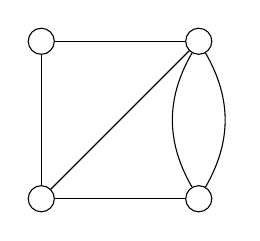
\begin{tikzpicture}[scale=2]
          \tikzset{vertex/.style = {shape=circle,draw,minimum size=0.5em}}
          \tikzset{edge/.style = {-,> = latex'}}

          \node[vertex] (1) at (0, 0) {};
          \node[vertex] (2) at (1, 0) {};
          \node[vertex] (3) at (1, -1) {};
          \node[vertex] (4) at (0, -1) {};

          \draw[edge] (1) to (2);
          \draw[edge, bend left] (2) to (3);
          \draw[edge, bend right] (2) to (3);
          \draw[edge] (3) to (4);
          \draw[edge] (1) to (4);
          \draw[edge] (2) to (4);
        \end{tikzpicture}
      \end{figure}
    \item 塗色擬陣:$E = E_1 \cup E_2 \cup \cdots \cup E_k$
      \[ \mathcal{I} = \{S \mid |S \cap E_i| \leq k_i\, \forall i \in [k]\} \]
    \item 均勻擬陣
      \[ \mathcal{I} = \{S \mid S \subseteq E, |S| \leq k\} \]
    \item 截斷擬陣
      \[ \mathcal{I}_k = \{S \mid S \in \mathcal{I}, |S| \leq k\} \]
  \end{itemize}
\end{frame}

\begin{frame}{\ctitle{Basis Exchange}}
  \onslide<1-> {
    \begin{lemma}[Weak Basis Exchange]
      令 $B_1$ 與 $B_2$ 是 $M$ 中的基底且 $B_1 \neq B_2$,則對於所有 $x \in B_1 \setminus B_2$,存在 $y \in B_2 \setminus B_1$ 使得 $(B_1 \setminus \{x\}) \cup \{y\}$ 是基底。
    \end{lemma}
  }
  \onslide<2-> {
    \begin{lemma}[Strong Basis Exchange]
      令 $B_1$ 與 $B_2$ 是 $M$ 中的基底且 $B_1 \neq B_2$,則對於所有 $x \in B_1 \setminus B_2$,存在 $y \in B_2 \setminus B_1$ 使得 $(B_1 \setminus \{x\}) \cup \{y\}$ 與
      $(B_2 \setminus \{y\}) \cup \{x\}$ 都是基底。
    \end{lemma}
  }
\end{frame}

\begin{frame}{\ctitle{最大權獨立集}}
  \begin{algorithm}[H]
    \KwData{擬陣 $M = (E, \mathcal{I})$、權重 $w: E \to \mathbb{R}_{\geq 0}$}
    \KwResult{最大權獨立集 $S \in \mathcal{I}$}

    \onslide<2-> {
      將 $E$ 照 $w$ 排序得到 $w(e_1) \geq w(e_2) \geq \ldots \geq w(e_n)$ \\
    }
    \onslide<3-> {
      $S \gets \emptyset$ \\
      \For{$i \gets 1$ \KwTo $n$} {
        \If{$S \cup \{e_i\} \in \mathcal{I}$} {
          $S \gets S \cup \{e_i\}$
        }
      }
    }
    \onslide<4-> {
      \Return $S$
    }
  \end{algorithm}
\end{frame}

\begin{frame}{\ctitle{最大權獨立集}}
  \begin{problem}
    有 $n$ 個數字 $a_1, a_2, \ldots, a_n$,以及 $w_1, w_2, \ldots, w_n$。請找出 $a$
    的一個子集,使得這個子集不管怎麼 XOR 都湊不出 $0$,且使得對應的 $w_i$ 總和最大。

    \begin{itemize}
      \item $1 \leq n \leq 10^5$
      \item $0 \leq a_i < 2^{30}$
    \end{itemize}
  \end{problem}
\end{frame}

\subsection{擬陣交}

\begin{frame}{\ctitle{Motivation}}
  \onslide<1-> {
    \begin{problem}[Faulty System]
      給定兩張 $n$ 點 $m$ 邊的無向圖,第 $i$ 條邊在第 $j$ 張圖連接點 $a_{ij}$ 與點 $b_{ij}$
    。請找出 $\{1, 2, \ldots, m\}$ 中最小的子集 $T$,使得加入編號在 $T$ 中的邊之後,兩張圖
      都變得連通。

      \begin{itemize}
        \item $1 \leq n, m \leq 300$
      \end{itemize}
    \end{problem}
  }
  \onslide<2-> {
    \begin{definition}[Matroid Intersection]
      對於擬陣 $M_1 = (E, \mathcal{I}_1)$ 以及 $M_2 = (E, \mathcal{I}_2)$,請找到

      \[ \argmax_{S \in \mathcal{I}_1 \cap \mathcal{I}_2}|S| \]
    \end{definition}
  }
\end{frame}

\begin{frame}{\ctitle{Greedy?}}
  \onslide<1-> {
    \begin{algorithm}[H]
      \KwData{擬陣 $M_1 = (E, \mathcal{I}_1), M_2 = (E, \mathcal{I}_2)$}
      \KwResult{最大擬陣交 $S \in \mathcal{I}_1 \cap \mathcal{I}_2$}

      $S \gets \emptyset$ \\

      \For{$i = 1$ \KwTo $n$} {
        \If{$S \cup \{e_i\} \in \mathcal{I}_1 \cap \mathcal{I}_2$} {
          $S \gets S \cup \{e_i\}$ \\
        }
      }

      \Return $S$
    \end{algorithm}
  }
  \onslide<2-> {
    \begin{figure}[H]
    \centering
    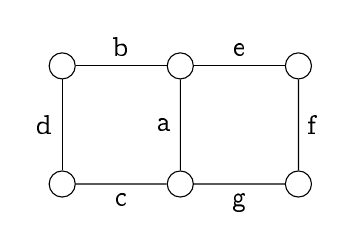
\begin{tikzpicture}[scale=1.5]
      \tikzset{vertex/.style = {shape=circle,draw,minimum size=0.5em}}
      \tikzset{edge/.style = {-,> = latex'}}
      \node[vertex] (1) at (0, 0) {};
      \node[vertex] (2) at (1, 0) {};
      \node[vertex] (3) at (2, 0) {};
      \node[vertex] (4) at (0, -1) {};
      \node[vertex] (5) at (1, -1) {};
      \node[vertex] (6) at (2, -1) {};

      \draw[edge] (1) to node[midway,above] {b} (2);
      \draw[edge] (2) to node[midway,above] {e} (3);
      \draw[edge] (1) to node[midway,left] {d} (4);
      \draw[edge] (4) to node[midway,below] {c} (5);
      \draw[edge] (2) to node[midway,left] {a} (5);
      \draw[edge] (5) to node[midway,below] {g} (6);
      \draw[edge] (3) to node[midway,right] {f} (6);
    \end{tikzpicture}
    \hspace{1em}
    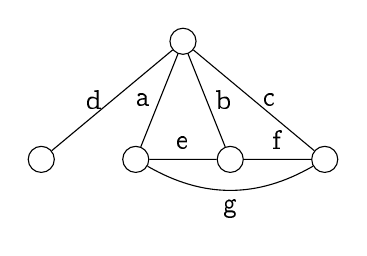
\begin{tikzpicture}[scale=1.5]
      \tikzset{vertex/.style = {shape=circle,draw,minimum size=0.5em}}
      \tikzset{edge/.style = {-,> = latex'}}
      \node[vertex] (1) at (0, 0) {};
      \node[vertex] (2) at (-1.2, -1) {};
      \node[vertex] (3) at (-0.4, -1) {};
      \node[vertex] (4) at (0.4, -1) {};
      \node[vertex] (5) at (1.2, -1) {};

      \draw[edge] (1) to node[midway,left] {d} (2);
      \draw[edge] (1) to node[midway,left] {a} (3);
      \draw[edge] (1) to node[midway,right] {b} (4);
      \draw[edge] (1) to node[midway,right] {c} (5);
      \draw[edge] (3) to node[midway,above] {e} (4);
      \draw[edge] (4) to node[midway,above] {f} (5);
      \draw[edge,bend right] (3) to node[midway,below] {g} (5);
    \end{tikzpicture}
  \end{figure}
  }
\end{frame}

\begin{frame}{\ctitle{Bipartite Matching}}
  \begin{figure}[H]
    \centering
    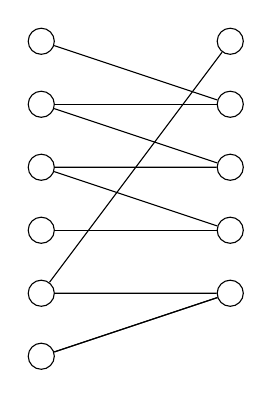
\begin{tikzpicture}[scale=0.8]
      \tikzset{vertex/.style = {shape=circle,draw,minimum size=0.5em}}
      \tikzset{edge/.style = {-,> = latex'}}
      \node[vertex] (x1) at (0, 0) {};
      \node[vertex] (x2) at (0, -1) {};
      \node[vertex] (x3) at (0, -2) {};
      \node[vertex] (x4) at (0, -3) {};
      \node[vertex] (x5) at (0, -4) {};
      \node[vertex] (x6) at (0, -5) {};
      \node[vertex] (y1) at (3, 0) {};
      \node[vertex] (y2) at (3, -1) {};
      \node[vertex] (y3) at (3, -2) {};
      \node[vertex] (y4) at (3, -3) {};
      \node[vertex] (y5) at (3, -4) {};
      \draw[edge] (x1) to (y2) {};
      \draw[edge] (x2) to (y2) {};
      \draw[edge] (x2) to (y3) {};
      \draw[edge] (x3) to (y3) {};
      \draw[edge] (x3) to (y4) {};
      \draw[edge] (x4) to (y4) {};
      \draw[edge] (x5) to (y1) {};
      \draw[edge] (x6) to (y5) {};
      \draw[edge] (x6) to (y5) {};
      \draw[edge] (x5) to (y5) {};
    \end{tikzpicture}
  \end{figure}

  \onslide<2-> {
    \[ \mathcal{I}_1 = \{E^\prime \subseteq E \mid |N_X(x) \cap E^\prime| \leq 1, \forall x \in X\} \]
    \[ \mathcal{I}_2 = \{E^\prime \subseteq E \mid |N_Y(y) \cap E^\prime| \leq 1, \forall y \in Y\} \]
  }
\end{frame}

\begin{frame}{\ctitle{Exchange Graph}}
  \onslide<1-> {
    \begin{figure}[H]
      \centering
      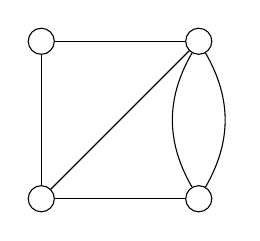
\begin{tikzpicture}[scale=2]
        \tikzset{vertex/.style = {shape=circle,draw,minimum size=0.5em}}
        \tikzset{edge/.style = {-,> = latex'}}

        \node[vertex] (1) at (0, 0) {};
        \node[vertex] (2) at (1, 0) {};
        \node[vertex] (3) at (1, -1) {};
        \node[vertex] (4) at (0, -1) {};

        \draw[edge] (1) to (2);
        \draw[edge, bend left] (2) to (3);
        \draw[edge, bend right] (2) to (3);
        \draw[edge] (3) to (4);
        \draw[edge] (1) to (4);
        \draw[edge] (2) to (4);
      \end{tikzpicture}
    \end{figure}
  }
  \onslide<2-> {
    \begin{lemma}
      對於兩個獨立集 $I_1$ 以及 $I_2$,則 $I_1 \setminus I_2 \subseteq I_1$ 以及
      $I_2 \setminus I_1 \subseteq E \setminus I_1$ 於 $\mathcal{D}_M(I_1)$ 中有完美匹
      配。
    \end{lemma}
  }
  \onslide<3-> {
    \begin{lemma}
      若 $I_1$ 是獨立集且 $\mathcal{D}_M(I_1)$ 中 $I_1 \setminus I_2$ 以及 
      $I_2 \setminus I_1$ 有\textbf{唯一}的完美匹配的話,則 $I_2$ 也是獨立集。
    \end{lemma}
  }
\end{frame}

\begin{frame}{\ctitle{Exchange Graph}}
  \begin{columns}
    \begin{column}{0.5\textwidth}
      \begin{itemize}
        \item $(s, x)$: $S \cup \{x\} \in \mathcal{I}_1$
        \item $(x, t)$: $S \cup \{x\} \in \mathcal{I}_2$
        \item $(x, y)$: $(S \setminus \{x\}) \cup \{y\} \in \mathcal{I}_1$
        \item $(y, x)$: $(S \setminus \{x\}) \cup \{y\} \in \mathcal{I}_2$
      \end{itemize}
    \end{column}
    \begin{column}{0.5\textwidth}
      \only<2> {
        \begin{figure}[H]
          \centering
          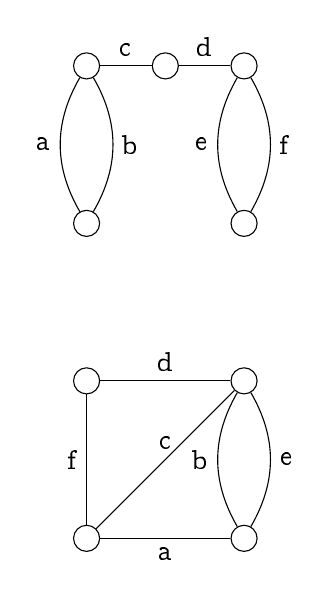
\begin{tikzpicture}[scale=2]
            \begin{scope}
              \tikzset{vertex/.style = {shape=circle,draw,minimum size=0.5em}}
              \tikzset{edge/.style = {-,> = latex'}}

              \node[vertex] (1) at (0, 0) {};
              \node[vertex] (2) at (0.5, 0) {};
              \node[vertex] (3) at (1, 0) {};
              \node[vertex] (4) at (0, -1) {};
              \node[vertex] (5) at (1, -1) {};

              \draw[edge] (1) to node[midway, above] {c} (2);
              \draw[edge] (2) to node[midway, above] {d} (3);
              \draw[edge, bend right] (1) to node[midway, left] {a} (4);
              \draw[edge, bend left] (1) to node[midway, right] {b} (4);
              \draw[edge, bend right] (3) to node[midway, left] {e} (5);
              \draw[edge, bend left] (3) to node[midway, right] {f} (5);
            \end{scope}
            \begin{scope}[shift=({0, -2})]
              \tikzset{vertex/.style = {shape=circle,draw,minimum size=0.5em}}
              \tikzset{edge/.style = {-,> = latex'}}

              \node[vertex] (1) at (0, 0) {};
              \node[vertex] (2) at (1, 0) {};
              \node[vertex] (3) at (1, -1) {};
              \node[vertex] (4) at (0, -1) {};

              \draw[edge] (1) to node[midway,above] {d} (2);
              \draw[edge, bend left] (2) to node[midway,right] {e} (3);
              \draw[edge, bend right] (2) to node[midway,left] {b} (3);
              \draw[edge] (3) to node[midway,below] {a} (4);
              \draw[edge] (1) to node[midway,left] {f} (4);
              \draw[edge] (2) to node[midway,above] {c} (4);
            \end{scope}
          \end{tikzpicture}
        \end{figure}
      }
    \end{column}
  \end{columns}
\end{frame}

\begin{frame}{\ctitle{Algorithm}}
  \begin{algorithm}[H]
    \KwData{擬陣 $M_1 = (E, \mathcal{I}_1), M_2 = (E, \mathcal{I}_2)$}
    \KwResult{最大擬陣交 $S \in \mathcal{I}_1 \cap \mathcal{I}_2$}

    \onslide<2-> {
      $S \gets \emptyset$ \\
      \onslide<3-> {
        \While{true} {
          $G_S \gets$ $S$ 的交換圖 \\
          $P \gets$ $G_S$ 中的最短 $s-t$ 路徑 \\

          \onslide<4-> {
            \If{$P = null$} {
              \Break
            }
          }

          \onslide<5-> {
            $S \gets S \triangle V(P)$
          }
        }
      }
      \Return $S$
    }
  \end{algorithm}
\end{frame}

\begin{frame}{\ctitle{Correctness}}
  \begin{theorem}
    \[ \max_{S \in \mathcal{I}_1 \cap \mathcal{I}_2}|S| = \min_{U \subseteq E}\{r_1(U) + r_2(E \setminus U)\} \]
  \end{theorem}
  \only<2> {
    \begin{theorem}
      若 $G_S$ 中沒有 $s$ 到 $t$ 的路徑,則存在 $U$ 使得 $r_1(U) = |S \cap U|$ 且 $r_2(U) = (S \cap (E \setminus U))$。
    \end{theorem}
  }
\end{frame}

\begin{frame}{\ctitle{Weighted Case}}
  \begin{algorithm}[H]
    \KwData{擬陣 $M_1 = (E, \mathcal{I}_1), M_2 = (E, \mathcal{I}_2)$、權重 $w: E \to \mathbb{R}_{\geq 0}$}
    \KwResult{最大權擬陣交 $S \in \mathcal{I}_1 \cap \mathcal{I}_2$}

    \onslide<2-> {
      $S \gets \emptyset$ \\

      \onslide<3-> {
        \While{true} {
          $G_S \gets$ $S$ 的交換圖 \\
          $l(e) \gets
            \begin{cases}
              +w(e), & e \in S \\
              -w(e), & e \not\in S \\
            \end{cases}$ \\
          \onslide<4-> {
            $P \gets$ $G_S$ 中的\emph{最短} $s-t$ 路徑 \\

            \onslide<5-> {
              \If{$P = null$} {
                \Break
              }
            }

            \onslide<6-> {
              $S \gets S \triangle V(P)$
            }
          }
        }
      }

      \Return $S$
    }
  \end{algorithm}
\end{frame}

\end{document}

\documentclass[standalone]{beamer}

\begin{document}
\section{其他主題}

\subsection{平面圖}

\begin{frame}{\ctitle{Definition}}
  \onslide<1-> {
    \begin{definition}
      一個圖 $G$ 是平面圖(planar graph)
      若 $G$ 可以被畫在平面上且沒有邊在非端點的地方交叉。一個將平面圖畫在平面上的方法稱為平版圖(plane graph)。
    \end{definition}
  }
  \onslide<2-> {
    \alt<3> {
      \begin{theorem}[Kuratowski's theorem]
        一個圖 $G$ 為平面圖若且唯若 $G$ 不包含 $K_5$ 或 $K_{3,3}$ 的細分子圖(subdivision)。
      \end{theorem}
      \begin{theorem}[Wagner's theorem]
        一個圖 $G$ 為平面圖若且唯若 $G$ 不包含 $K_5$ 或 $K_{3,3}$ 的次圖(minor)。
      \end{theorem}
    } {
      \begin{figure}[H]
        \centering
        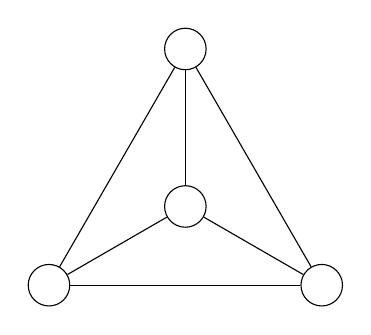
\begin{tikzpicture}[scale=2]
        \tikzset{vertex/.style = {shape=circle,draw,minimum size=1.5em}}
        \tikzset{edge/.style = {-,> = latex'}}
        \node[vertex] (a) at (0, 0) {};
        \node[vertex] (b) at (0, 1) {};
        \node[vertex] (c) at (0.866, -0.5) {};
        \node[vertex] (d) at (-0.866, -0.5) {};

        \draw[edge] (a) to (b);
        \draw[edge] (a) to (c);
        \draw[edge] (a) to (d);
        \draw[edge] (b) to (c);
        \draw[edge] (b) to (d);
        \draw[edge] (c) to (d);
        \end{tikzpicture}
        \hspace{0.1\textwidth}
        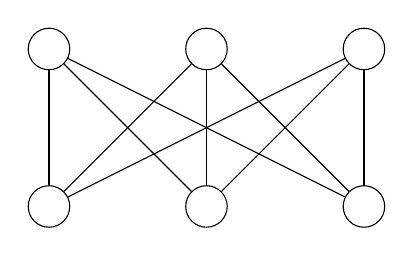
\begin{tikzpicture}[scale=2]
        \tikzset{vertex/.style = {shape=circle,draw,minimum size=1.5em}}
        \tikzset{edge/.style = {-,> = latex'}}
        \node[vertex] (x1) at (0, 0) {};
        \node[vertex] (x2) at (1, 0) {};
        \node[vertex] (x3) at (2, 0) {};
        \node[vertex] (y1) at (0, -1) {};
        \node[vertex] (y2) at (1, -1) {};
        \node[vertex] (y3) at (2, -1) {};

        \draw[edge] (x1) to (y1);
        \draw[edge] (x1) to (y2);
        \draw[edge] (x1) to (y3);
        \draw[edge] (x2) to (y1);
        \draw[edge] (x2) to (y2);
        \draw[edge] (x2) to (y3);
        \draw[edge] (x3) to (y1);
        \draw[edge] (x3) to (y2);
        \draw[edge] (x3) to (y3);
        \end{tikzpicture}
      \end{figure}
    }
  }
\end{frame}

\begin{frame}{\ctitle{尤拉公式}}
  \onslide<1-> {
    \begin{theorem}[尤拉公式]
      對於一個\emph{連通}的平面圖 $G$,若 $G$ 有 $V$ 個點、$E$ 條邊以及 $F$ 個面,則 $V - E + F = 2$。
    \end{theorem}
  }
  \onslide<2-> {
    \begin{theorem}[尤拉公式]
      對於一個的平面圖 $G$,若 $G$ 有 $V$ 個點、$E$ 條邊、 $F$ 個面以及 $C$ 個連通塊,則 $V - E + F = C + 1$。
    \end{theorem}
  }
  \onslide<3-> {
    \begin{corollary}
      一個 $n$ 點的連通平面圖至多有 $3n - 6$ 條邊。
    \end{corollary}
  }
\end{frame}

\begin{frame}{\ctitle{四/五色定理}}
  \onslide<1-> {
    \begin{theorem}[四色定理]
      平面圖可以被四著色。
    \end{theorem}
  }
  \onslide<2-> {
    \begin{theorem}[五色定理]
      平面圖可以被五著色。
    \end{theorem}
  }
  \onslide<3-> {
    \begin{problem}[Four coloring]
      給定平面上 $n$ 個點的座標 $(x_i, y_i)$ 以及一些連接他們的邊,保證邊不相交(所以是平面圖)
      ,並且每條邊不是水平、垂直、就是 45 度。也就是說,對於邊 $(u, v)$,一定有 $x_u = x_v$、
      $y_u = y_v$ 或是 $|x_u - x_v| = |y_u - y_v|$。求這張圖上的一個四塗色。

      \begin{itemize}
        \item $1 \leq n \leq 10000$
      \end{itemize}
    \end{problem}
  }
\end{frame}

\subsection{環與割}

\begin{frame}{\ctitle{Motivation}}
  \begin{problem}[Counting Cycles]
    給定一個 $n$ 點 $m$ 邊的簡單連通無向圖,請輸出圖中有幾個簡單環。

    \begin{itemize}
      \item $3 \leq n \leq 10^5$
      \item $n - 1 \leq m \leq n + 15$
    \end{itemize}
  \end{problem}

  \onslide<2> {
    \begin{problem}[Planar Max Cut]
      給定一個平面圖 $G$,找到一個點集 $S$ 使得連接 $S$ 與 $V(G) \setminus S$ 的邊數最多。

      \begin{itemize}
        \item $1 \leq n \leq 200$
        \item $1 \leq m \leq 1000$
      \end{itemize}
    \end{problem}
  }
\end{frame}

\begin{frame}{\ctitle{Vector Space}}
  \onslide<1-> {
    \begin{definition}[Cut Space]
      $G = (V, E)$ 中的割空間定義為 $\{\eta(v) \mid v \in V\}$ 所生成的子空間。
    \end{definition}
  }
  \onslide<2-> {
    \begin{definition}[Cycle Space]
      $G = (V, E)$ 中的環空間定義為

      \[ \{E^\prime \subseteq E \mid G[E^\prime] \text{ 中所有點的度數都是偶數}\} \]
    \end{definition}
  }
\end{frame}

\begin{frame}{\ctitle{Basis}}
  \onslide<1-> {
    \begin{lemma}
      $\{\eta(v_2), \eta(v_3), \ldots, \eta(v_n)\}$ 為割空間的一組基底。
    \end{lemma}
  }
  \onslide<2-> {
    \begin{definition}[基本環]
      給定 $G = (V, E)$ 以及 $G$ 的一棵生成樹 $T$,對於\textbf{非樹邊} $e \in E \setminus T$,
      $e = (u, v)$ 對應的基本環(fundamental cycle)$C_e$ 為 $e$ 與 $T$ 中 $u$ 到 $v$ 的
      路徑所構成的環。
    \end{definition}
  }
  \onslide<3-> {
    \begin{lemma}
      令 $T$ 為 $G$ 的一棵生成樹,則 $\{\eta(C_e) \mid e \notin T\}$ 是環空間的一組基底。
    \end{lemma}
  }
\end{frame}

\begin{frame}{\ctitle{Example}}
  \begin{problem}[Counting Cycles]
    給定一個 $n$ 點 $m$ 邊的簡單連通無向圖,請輸出圖中有幾個簡單環。

    \begin{itemize}
      \item $3 \leq n \leq 10^5$
      \item $n - 1 \leq m \leq n + 15$
    \end{itemize}
  \end{problem}
\end{frame}

\begin{frame}{\ctitle{Planar Graph}}
  \onslide<1-> {
    \begin{problem}[$st$ Min Cut on Planar Graph 簡化版]
      給定一個平面圖 $G = (V, E)$ 以及 $s, t \in V$,找到一個點集 $S$ 使得 $s \in S$ 且 $t \in V \setminus S$ 使得 $S$ 與 $V \setminus S$ 的邊數\emph{最少}。

      \begin{itemize}
        \item 保證 $s$ 與 $t$ 位於同一個面上
      \end{itemize}
    \end{problem}
  }
  \onslide<2-> {
    \begin{figure}
      \begin{tikzpicture}[scale=0.7]
        \foreach \i in {0,...,4} {
          \draw (\i,0) -- (\i,4);
        }
        \foreach \i in {0,...,4} {
          \draw (0,\i) -- (4,\i);
        }

        \node at (-0.2, -0.2) {$s$};
        \node at (4.2, 4.2) {$t$};
      \end{tikzpicture}
    \end{figure}
  }
\end{frame}

\begin{frame}{\ctitle{Planar Graph}}
  \onslide<1-> {
    \begin{definition}
      對於平版圖 $G = (V, E)$(也就是平面圖加上一個嵌於平面的方法),$G$ 的對偶圖(Dual)定義為
      $G^{*} = (F, E^{*)})$,其中 $F$ 為 $G$ 的面,而對於所有 $E$ 中的邊 $e$,若在 $G$ 中
      $e$ 兩側的面分別為 $f_1$ 與 $f_2$,則 $(f_1, f_2) \in E^{*}$。
    \end{definition}
  }
  \onslide<2-> {
    \alt<3> {
      \begin{theorem}
        $G$ 的環空間等於 $G^{*}$ 的割空間,且 $G$ 的割空間等於 $G^{*}$ 的環空間。
      \end{theorem}
    } {
      \begin{figure}[H]
        \centering
        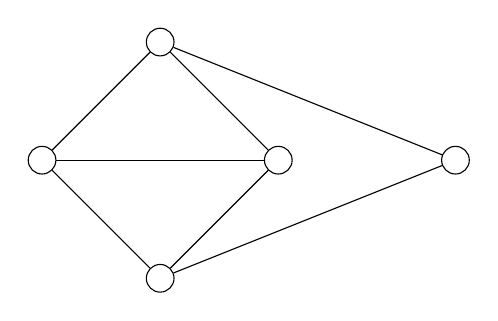
\begin{tikzpicture}[scale=1.5]
          \tikzset{vertex/.style = {shape=circle,draw,minimum size=1em}}
          \tikzset{edge/.style = {-,> = latex'}}
          \node[vertex] (a) at (0, 0) {};
          \node[vertex] (b) at (-1, -1) {};
          \node[vertex] (c) at (1, -1) {};
          \node[vertex] (d) at (0, -2) {};
          \node[vertex] (e) at (2.5, -1) {};

          \draw[edge] (a) to (b);
          \draw[edge] (a) to (c);
          \draw[edge] (b) to (d);
          \draw[edge] (c) to (d);
          \draw[edge] (e) to (a);
          \draw[edge] (e) to (d);
          \draw[edge] (b) to (c);
        \end{tikzpicture}
      \end{figure}
    }
  }
\end{frame}

\begin{frame}{\ctitle{Planar Max Cut}}
  \begin{problem}[Planar Max Cut]
    給定一個平面圖 $G$,找到一個點集 $S$ 使得連接 $S$ 與 $V(G) \setminus S$ 的邊數最多。

    \begin{itemize}
      \item $1 \leq n \leq 200$
      \item $1 \leq m \leq 1000$
    \end{itemize}
  \end{problem}
\end{frame}

\subsection{推廣樹 DP}

\begin{frame}{\ctitle{Tree Decomposition}}
  \begin{definition}[樹分解]
    對於圖 $G$,$G$ 的一個樹分解(Tree Decomposition)為 $(X, T)$,其中

    \begin{itemize}
      \item $X = \{X_1, X_2, \ldots, X_k\}$ 是一個 $G$ 的點集組成的序列,也就是
        $X_i \subseteq V(G)$($X_v$ 通常被稱為一個 bag)
      \item $T$ 是以 $X$ 為節點的一棵樹
    \end{itemize}

    \onslide<2-> {
      使得

      \begin{itemize}
        \item $X_1 \cup X_2 \cup \cdots \cup X_k = V(G)$,也就是 $G$ 中的每個節點都至少在
          一個 $X_i$ 中
        \item 對於所有 $G$ 中的邊 $(u, v)$,存在 $X_i$ 使得 $u$ 跟 $v$ 都在 $X_i$ 中
        \item 對於所有 $G$ 中的節點 $v$,包含 $v$ 的 $X_i$ 在 $T$ 中是一個連通子樹
      \end{itemize}
    }
  \end{definition}
\end{frame}

\begin{frame}{\ctitle{Tree Decomposition}}
  \begin{figure}[H]
    \centering
    \begin{tikzpicture}[scale=2]
      \tikzset{vertex/.style = {shape=circle,draw,minimum size=1.5em}}
      \tikzset{edge/.style = {-,> = latex'}}
      \node[vertex] (a) at (0, 0) {$1$};
      \node[vertex] (b) at (1, 0) {$2$};
      \node[vertex] (c) at (2, 0) {$3$};
      \node[vertex] (d) at (0, -1) {$4$};
      \node[vertex] (e) at (2, -1) {$5$};
      \node[vertex] (f) at (0, -2) {$6$};
      \node[vertex] (g) at (1, -2) {$7$};
      \node[vertex] (h) at (2, -2) {$8$};

      \draw[edge] (a) to (b);
      \draw[edge] (c) to (b);
      \draw[edge] (a) to (d);
      \draw[edge] (b) to (d);
      \draw[edge] (b) to (e);
      \draw[edge] (c) to (e);
      \draw[edge] (d) to (f);
      \draw[edge] (f) to (g);
      \draw[edge] (g) to (h);
      \draw[edge] (e) to (h);
      \draw[edge] (d) to (g);
      \draw[edge] (e) to (g);
      \draw[edge] (b) to (g);
    \end{tikzpicture}
  \end{figure}
\end{frame}

\begin{frame}{\ctitle{Good Tree Decomposition}}
  \begin{itemize}
    \item Introduce node $v$:
      \[ X_v = X_u \cup \{x\} \]
    \item Forget node $v$:
      \[ X_v = X_u \setminus \{x\} \]
    \item Join node $v$:
      \[ X_v = X_{u_1} = X_{u_2} \]
  \end{itemize}
\end{frame}

\begin{frame}{\ctitle{Maximum Weighted Independent Set}}
  \onslide<1-> {
    \begin{itemize}
      \item Introduce node $v$:
        \onslide<2-> {
          \[ dp(v, S) =
            \begin{cases}
              dp(u, S), & x \notin S \\
              w(x) + dp(u, S \setminus \{x\}), & \text{若 $S$ 是獨立的} \\
              -\infty, & \text{otherwise}
            \end{cases}
          \]
        }
      \item Forget node $v$:
        \onslide<3-> {
          \[
            dp(v, S) = \max(dp(u, S), dp(u, S \cup \{x\}))
          \]
        }
      \item Join node $v$:
        \onslide<4-> {
          \[
            dp(v, S) = dp(u_1, S) + dp(u_2, S) - w(S)
          \]
        }
    \end{itemize}
  }
\end{frame}

\end{document}


\end{document}

